\documentclass{article}
\usepackage[T1]{fontenc}
\usepackage{lmodern}
\usepackage{graphicx}
\usepackage{amsmath,amssymb}
\usepackage[a4paper,margin=2cm]{geometry}
\usepackage[absolute,overlay]{textpos}
\setlength{\TPHorizModule}{1mm}
\setlength{\TPVertModule}{1mm}
\usepackage[indonesian]{babel}
\usepackage{hyperref}
\setlength{\emergencystretch}{2em}
% unit: Halaman 30

\begin{document}

% === Halaman 30 (llm) ===

\vspace{98.01mm}

$C_1$ diperoleh sebagai berikut:
\[ P_1 \oplus C_0 = 1010 \oplus 0000 = 1010 \]

% deskripsi: Diagram blok proses enkripsi cipher feedback mode (CFB) yang menunjukkan aliran data melalui fungsi E dan operasi XOR dengan plaintext P untuk menghasilkan ciphertext C.
% bbox normalisasi: [0.5200, 0.3500, 0.9700, 0.6800]
\begin{textblock*}{94.50mm}(109.20mm,103.95mm)
\noindent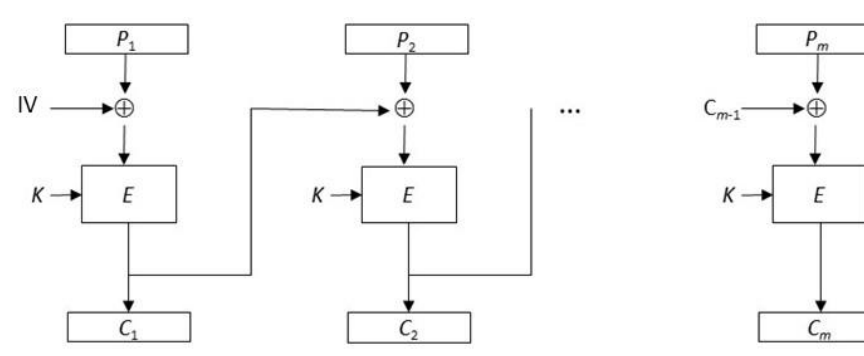
\includegraphics[width=94.50mm,height=98.01mm]{../../images/llm/page_030_img_01.png}%
\end{textblock*}

\end{document}
